\documentclass[
	openany,
	10pt,
	parindent=0
] {article}

\usepackage[a5paper,top=2cm,bottom=2cm,left=1.5cm,right=1.5cm]{geometry}

\usepackage{import}
\usepackage[T2A]{fontenc}
\usepackage[english,russian]{babel}

\usepackage{amsmath}
\usepackage{amsfonts}
\usepackage{amssymb}
\usepackage{amsthm}

\usepackage{braket}
\usepackage{blkarray}
\usepackage{graphics}
\usepackage{subcaption}

\usepackage{titlesec}
\usepackage{enumitem}
\usepackage{parskip}
\usepackage{setspace}

\setstretch{1}
\setlength{\parindent}{0pt}

\usepackage{tikz}
	\usetikzlibrary{arrows.meta}
	\usetikzlibrary{graphs, graphs.standard}

\tikzset{
	node distance={12mm}, minimum size={5mm}, inner sep={0mm}, main/.style = {draw, circle}
}

\titleformat{\section}[block]{\normalfont\bfseries\normalsize}{\thesection}{0.3em}{}
\titlespacing*{\section}{0em}{0pt}{10pt}

\newtheoremstyle{custom} % Имя стиля
  {3pt}      % Отступ сверху
  {3pt}      % Отступ снизу
  {\normalsize} % Шрифт для тела теоремы
  {}         % Величина отступа
  {\bfseries}% Шрифт заголовка теоремы
  {}         % Знак препинания после заголовка теоремы
  { }        % Пробел после заголовка теоремы
  {\thmname{#1}\thmnote{ \bfseries#3}} % Спецификация заголовка теоремы

\theoremstyle{custom}
\newtheorem{theorem}{Теорема:}[section]
\newtheorem{definition}{Опр:}[section]
\makeatletter
\renewenvironment{proof}[1][\proofname]{\par
  \pushQED{\qed}%
  \normalfont \topsep6\p@\@plus6\p@\relax
  \trivlist
  \item[\hskip\labelsep
        \bfseries
    Док-во:\@addpunct{}]%
    \ignorespaces
}{%
  \popQED\endtrivlist\@endpefalse
}
\makeatother


\newcommand*{\titleASU}{\begingroup
	\begin{center}
        \large
		Санкт-Петербургский государственный электротехнический университет
		имени В. И. Ленина "ЛЭТИ"
		\vfill
		билеты \\ 
		\huge{\textbf{КОМБИНАТОРИКА И ТЕОРИЯ ГРАФОВ}} \\
        \vspace*{200pt}
        \large
        Студент: \hfill Придчин В.Е.\\
        Группа: \hfill 2308 \\
        Лектор: \hfill Зяблицева Л.
		\vfill
    \LaTeX
    \vfill
		Санкт-Петербург \\ 2024
		\newpage
	\end{center}
\endgroup}

\begin{document}
    \begin{titlepage}
        \titleASU
    \end{titlepage}

    \setcounter{page}{2}

    \section{Основные определения теории графов. Смежность и инцидентность вершин и ребер графа. 
Степени вершин в графе и орграфе. Теоремы о сумме степеней вершин в графе и орграфе. 
Матрицы смежности и инцидентности. Найти матрицы смежности и инцидентности указанного 
графа.}

$V$ -- множество вершин. \\
$E$ -- множество пар вида $(u, v): u, v \in V$ (множество ребер).

\begin{definition}
    Графом -- называют совокупность 2-ух множеств непустого множества E
	\begin{equation*}
		E = \{(u, v): u, v \in V\}, \; G(V, E) - \textit{обозначение графа}
	\end{equation*}
\end{definition}

\begin{definition}
    Петля -- пара вида $(v,v)$ в множестве $E$.
\end{definition}

\begin{definition}
    Кратные ребра -- одинаковые пары в множестве $E$. Количество кратных ребер - кратность ребра.
\end{definition}

\noindent
Существуют следующие виды графов:
\begin{enumerate}[left=0.0em, labelsep=1em, topsep=0.5em, itemsep=0pt, parsep=0.5em]
    \item Псевдограф -- в графе могут быть и \textit{кратные ребра}, и \textit{петли}.
    \item Мультиграф -- в графе есть \textit{кратные ребра}, но нет \textit{петель}.
    \item Простой граф -- отсутствуют и \textit{кратные ребра} и \textit{петли}.
\end{enumerate}

\begin{definition}
    Ориентированный граф (орграф) -- граф с ориентированными ребрами.
\end{definition}

\begin{definition}
    Если $e=(u,v)$ -- ребро неориентированного графа, то $u, v$ - концы ребра.
\end{definition}

\begin{definition}
    Если $e=(u,v)$ -- ребро (дуга) ориентированного графа, то $u$ - начало ребра, $v$ - конец ребра.
\end{definition}

\begin{definition}
    $a, b \text{ \textit{смежные}} \Leftrightarrow e=(u,v)$.
\end{definition}

\begin{definition}
    $u, v \text{ \textit{инцидентны ребру }} e \Leftrightarrow e=(u,v)$.
\end{definition}

\begin{definition}
	Степенью вершины $v$ неориентированного графа называется количество ребер инцидентных данной вершине, $\delta(v)$ (петлю считают два \mbox{раза}).
\end{definition}

\begin{minipage}{0.55\textwidth}
	\centering
	\begin{tikzpicture}
		\node[main] (1) {$1$};
		\node[main] (3) [above right of=1] {$3$};
		\node[main] (5) [below right of=3] {$5$};
		\node[main] (2) [above of=5] {$2$};
		\node[main] (4) [below left of=5] {$4$};
		
		\draw (3) to [out=90,in=180,looseness=5] (3);
		\draw (1) -- (3);
		\draw (3) -- (5);
		\draw (1) -- (5);
		\draw (4) -- (5);
	\end{tikzpicture}
\end{minipage}
\begin{minipage}{0.3\textwidth}
	$\begin{aligned}
		&\delta(1) = 2 & \delta(4) &= 1 \\
		&\delta(2) = 0 & \delta(5) &= 3 \\
		&\delta(3) = 4 & \Rightarrow sum &= 10
	\end{aligned}$
\end{minipage}

\begin{theorem}
    Сумма степеней вершин неориентированного графа равна удвоенному числу ребер
	\begin{align*}
		\sum_{u \in V}\delta(v)=2r, \textit{ где r - число ребер}
	\end{align*}
\end{theorem}

\begin{proof}
    Теорема справедлива, так как вклад каждого ребра равен двум.
\end{proof}

\begin{definition}
    Если степень вершины равна нулю, то вершина \textit{изолированная}, \\ $\delta(v)=0$.
\end{definition}

\begin{definition}
    Если степень вершины равна единице, то вершина \textit{висячая}, $\delta(v)=1$
\end{definition}

\begin{definition}
    Полустепенью исхода(захода) вершина $v$ ориентированного графа называют количество ребер исходящих(заходящих) в данную вершину.
    \begin{tikzpicture}[baseline={(A.base)}]
		\node [text width=5cm] (A) at (0,0) {$\delta^-(v)$ -- полустепень исхода\\
			$\delta^+(v)$ -- полустепень захода};
	\end{tikzpicture}
\end{definition}

\begin{theorem}
	Для орграфа справедливо равенство
	\begin{align*}
		\sum_{u \in V}\delta^-(v)=\sum_{u \in V}\delta^+(v)=r, \textit{ где r -- число ребер}
	\end{align*}
\end{theorem}

\begin{minipage}{0.5\textwidth}
	\centering
	\begin{tikzpicture}
		\node[main] (a) {$a$};
		\node[main] (d) [right of=a] {$d$};
		\node[main] (b) [above of=d] {$b$};
		\node[main] (c) [right of=b] {$c$};
		\node[main] (e) [below of=d] {$e$};
		
		\draw[-{Stealth[length=2mm]}] (e) to [out=270,in=360,looseness=5] (e);
		\draw[-{Stealth[length=2mm]}] (a) -- (d);
		\draw[-{Stealth[length=2mm]}] (a) -- (e);
		\draw[-{Stealth[length=2mm]}] (a) -- (b);
		\draw[-{Stealth[length=2mm]}] (b) -- (c);
		\draw[-{Stealth[length=2mm]}] (e) -- (d);
	\end{tikzpicture}
\end{minipage}
\begin{minipage}{0.5\textwidth}
	$\begin{aligned}
		\delta^-(a) &= 3 &\delta^+(a) = 0 \\
		\delta^-(b) &= 1 &\delta^+(b) = 1 \\
		\delta^-(c) &= 0 &\delta^+(c) = 1 \\
		\delta^-(d) &= 0 &\delta^+(d) = 2 \\
		\delta^-(e) &= 2 &\delta^+(e) = 2 \\
		\sum\delta^-(v) &= 6; \; &\sum\delta^+(v) = 6 \\
	\end{aligned}$
\end{minipage}

\begin{definition}
    Матрицей смежности графа(орграфа) называют квадратную матрицу размерностью $n$, где $n=|v|$ (мощность множества вершин), в котором $a_{ij}=k$, где $k$ - число ребер $(v_i,v_j)$
\end{definition}

\begin{definition}
    Пусть $G(V,E)$ -- неориентированный граф. Матрицей инцидентности неориентированного графа называется матрица $B$ размером $n*r$, $|v| = n, |E| = r$, где каждый элемент матрицы:
	\begin{align*}
		b_{ij}=\left\{\begin{array}{l}
			1, \text{ если $v_i$ инцидентно ребру $e_j$}
			\\ 
			0, \text{ иначе}
		\end{array}\right.
	\end{align*}
\end{definition}
\noindent
Такая матрица будет симметричной.

\begin{definition}
    Пусть $G(V,E)$ -- ориентированный граф. Матрицей инцидентности ориентированного графа называется матрица $B$ размером $n*r$, $|v| = n, |E| = r$, где каждый элемент матрицы:
	\begin{align*}
		b_{ij}=\left\{\begin{array}{l}
			-1, \text{ если ребро $e_j$ выходит из $v_i$}
			\\
			1, \text{ если ребро $e_j$ входит из $v_i$}
			\\ 
			0, \text{ иначе}
		\end{array}\right.
	\end{align*}
\end{definition}

Если есть петля, то на соответствующее место ставят любое число.

Поиск матрицы смежности $A$ и инцидентности $B$ для неориентированного графа:
\begin{figure}[ht]
	\centering
	\begin{minipage}[b]{0.45\linewidth}
		\centering
		\begin{tikzpicture}[node distance=30mm]
			\node[main] (a) {$a$};
			\node[main] (b) [above of=a] {$b$};
			\node[main] (c) [right of=b] {$c$};
			\node[main] (d) [below of=c] {$d$};
			
			\draw[] (a) -- node[midway, left]{$e_1$} (b);
			\draw[] (a) -- node[midway, below right]{$e_2$} (c);
			\draw[] (b) to [out=30, in= 150] node[midway, above]{$e_3$} (c);
			\draw[] (b) -- node[midway, below]{$e_4$} (c);
			\draw[] (c) -- node[midway, right]{$e_5$} (d);
			\draw[] (d) to [out=270,in=360,looseness=5] node[midway, below right]{$e_6$} (d);
		\end{tikzpicture}
	\end{minipage}
	\begin{minipage}[b]{0.45\linewidth}
		\begin{flalign*}
			&A =
			\begin{blockarray}{ccccc}
				& a & b & c & d \\
				\begin{block}{c(cccc)}
					a & 0 & 1 & 1 & 0 \\
					b & 1 & 0 & 2 & 0 \\
					c & 1 & 2 & 0 & 1 \\
					d & 0 & 0 & 1 & 1 \\
				\end{block}
			\end{blockarray} \\
			&B =
			\begin{blockarray}{ccccccc}
				& e_1 & e_2 & e_3 & e_4 & e_5 & e_6 \\
				\begin{block}{c(cccccc)}
					a & 1 & 1 & 0 & 0 & 0 & 0\\
					b & 1 & 0 & 1 & 1 & 0 & 0\\
					c & 0 & 1 & 1 & 1 & 1 & 0\\
					d & 0 & 0 & 0 & 0 & 1 & 1\\
				\end{block}
			\end{blockarray}
		\end{flalign*}
	\end{minipage}
\end{figure}

\newpage
Поиск матрицы смежности $A$ и инцидентности $B$ для ориентированного графа:
\begin{figure}[ht]
	\centering
	\begin{minipage}[b]{0.40\linewidth}
		\begin{tikzpicture}[node distance=22mm, minimum size=17, remember picture, overlay]
			\node[main] (a) at ([xshift=-5.2cm, yshift=5cm]current page) {$a$};
			\node[main] (b) [above right of=a] {$b$};
			\node[main] (c) [right of=b] {$c$};
			\node[main] (d) [right of=a] {$d$};
			\node[main] (e) [below right of=a] {$e$};
			
			\draw[-{Stealth[length=2mm]}] (e) to [out=270,in=360,looseness=5] node[midway, below]{$e_6$}(e);
			\draw[-{Stealth[length=2mm]}] (a) -- node[midway, above]{$e_2$} (d);
			\draw[-{Stealth[length=2mm]}] (a) -- node[midway, below left]{$e_3$} (e);
			\draw[-{Stealth[length=2mm]}] (a) -- node[midway, left]{$e_1$} (b);
			\draw[-{Stealth[length=2mm]}] (b) -- node[midway, below]{$e_4$} (c);
			\draw[-{Stealth[length=2mm]}] (e) -- node[midway, left]{$e_5$} (d);
		\end{tikzpicture}
		\hfil
	\end{minipage}
	\begin{minipage}[t]{0.45\linewidth}
		\vspace*{-5mm}
		\begin{flalign*}
			&A =
			\begin{blockarray}{cccccc}
				& a & b & c & d & e\\
				\begin{block}{c(ccccc)}
					a & 0 & 1 & 0 & 1 & 1 \\
					b & 0 & 0 & 1 & 0 & 0 \\
					c & 0 & 0 & 0 & 0 & 0 \\
					d & 0 & 0 & 0 & 0 & 0 \\
					e & 0 & 0 & 0 & 1 & 1 \\
				\end{block}
			\end{blockarray} \\
			&B =
			\begin{blockarray}{ccccccc}
				& e_1 & e_2 & e_3 & e_4 & e_5 & e_6 \\
				\begin{block}{c(cccccc)}
					a & -1 & -1 & -1 & 0 & 0 & 0\\
					b & 1 & 0 & 0 & -1 & 0 & 0\\
					c & 0 & 0 & 0 & 1 & 0 & 0\\
					d & 0 & 1 & 0 & 0 & 1 & 0\\
					e & 0 & 0 & 1 & 0 & -1 & 1\\
				\end{block}
			\end{blockarray}
		\end{flalign*}
	\end{minipage}
\end{figure}
	\section{Полные и двудольные графы. Число ребер в полном графе с n вершинами и в полном 
двудольном графе (вывод формул).}

\begin{definition}
    \textit{Полный граф} -- простой неориентированный граф у которого любые две вершины смежны.
\end{definition}

\begin{tikzpicture}
    % K1
    \graph[nodes={draw, circle}] { subgraph K_n [n=1,clockwise,radius=0.8mm] };
    \node at (0,-1.5) {$K_1$};
  
    % K2
    \begin{scope}[xshift=6.5em]
        \graph[nodes={draw, circle}] { subgraph K_n [n=2,clockwise,radius=0.8cm] };
      \node at (0,-1.5) {$K_2$};
    \end{scope}
  
    % K3
    \begin{scope}[xshift=14em]
        \graph[nodes={draw, circle}] { subgraph K_n [n=3,clockwise,radius=0.8cm] };
      \node at (0,-1.5) {$K_3$};
    \end{scope}
  
    % K4
    \begin{scope}[xshift=22em]
        \graph[nodes={draw, circle}] { subgraph K_n [n=4,clockwise,radius=0.8cm] };
      \node at (0,-1.5) {$K_4$};
    \end{scope}
  
    % K5
    \begin{scope}[xshift=30em]
        \graph[nodes={draw, circle}] { subgraph K_n [n=5,clockwise,radius=0.8cm] };
      \node at (0,-1.5) {$K_5$};
    \end{scope}
  \end{tikzpicture}

Количество полных ребер в графе $K_n = C_n^2= \frac{n!}{2!(n-2)!} = \frac{n(n-1)}{2}$.

\begin{definition}
    \textit{Двудольный граф} -- граф, если его множество вершин $V$ можно разделить на подмножество $V_1$ и $V_2$ такое что:
	\begin{tikzpicture}[baseline={(A.base)}]
		\node [text width=2cm] (A) at (0,0) {$V_1 \cap V_2 = \varnothing$\\
			$V_1 \cup V_2 = V$};
	\end{tikzpicture}
\end{definition}

Смежными могут быть только вершины из разных долей графа.

\begin{center}
\begin{tikzpicture}
	\graph[nodes={draw, circle}] {
		subgraph I_nm [V={1, 2, 3}, W={4, 5}];
		
		1 -- { 4, 5};
		2 -- { 4, 5};
		3 -- { 5 }
	};

    \node[anchor=west] at (2, -0.5) {
        \begin{minipage}{4cm}
        \begin{align*}
            V &= \{1, 2, 3, 4, 5\} \\
            V_1 &= \{1, 2, 3\} \\
            V_2 &= \{4, 5\}
        \end{align*}
        \end{minipage}
    };
\end{tikzpicture}
\end{center}

\begin{definition}
    \textit{Полный двудольный граф} -- каждая вершина одной доли соединяется с другой.
    $K_{t_1, k_2}$, где ${t_1, k_2}$ -- количество вершин в долях графа.
\end{definition}

\begin{center}
\begin{tikzpicture}
	\graph[nodes={draw, circle}] {
		subgraph I_nm [V={1, 2, 3}, W={4, 5, 6}];
		
		1 -- { 4, 5, 6};
		2 -- { 4, 5, 6};
		3 -- { 4, 5, 6}
	};

    \node[anchor=west] at (2, -0.5) {
        \begin{minipage}{4cm}
        \begin{align*}
            K_{3,3}\\
            V &= \{1, 2, 3, 4, 5, 6\} \\
            V_1 &= \{1, 2, 3\} \\
            V_2 &= \{4, 5, 6\}
        \end{align*}
        \end{minipage}
    };
\end{tikzpicture}
\end{center}

В полном двудольном графе содержится $t_1 \cdot t_2$ ребер.
	\section{Изоморфизм и гомеоморфизм графов. Примеры изоморфных и гомеоморфных графов. Способы 
проверки изоморфизма графов. Инварианты графа. Дополнение графа, проверка изоморфизма 
графов с помощью дополнений. Выяснить, являются ли графы G1 и G2 изоморфными, 
гомеоморфными.}

\begin{definition}
    \textit{Изоморфизм графов} -- биективное отображение $\varphi: V_1 \rightarrow V_2$, такое что:
    \begin{align*}
        (\forall u,v \in V)((u,v) \in E_1) \Leftrightarrow (\varphi(u),\varphi(v)) \in E_2
    \end{align*}
\end{definition}

Изоморфные графы обозначаются: $G_1 \cong G_2$

Изоморфные объекты \textit{не различимы} с точки зрения математики. Это экземпляры
одного и того же математического объекта. Изоморфные объекты имеют одинаковое
число элементов и свойств.

Изоморфизм графов можно определить:
\begin{enumerate}[left=0.0em, labelsep=1em, topsep=0.0em, itemsep=0pt, parsep=0.5em]
    \item По определению (найдя биективное отображение множества вершин,
    сохраняющее смежность)
    \item Перерисовав один из графов так, чтобы изображение совпало с другим
    графом
    \item Сравнив матрицы смежности графов
\end{enumerate}

\begin{theorem}
    Графы изоморфны тогда и только тогда, когда матрицу смежности
одного из них можно получить из матрицы смежности другого путём
одновременной перестановки местами $i$-ой и $j$-ой строк и столбцов.
\end{theorem}

Пример изоморфных графов:
\begin{figure}[h]
    \centering
    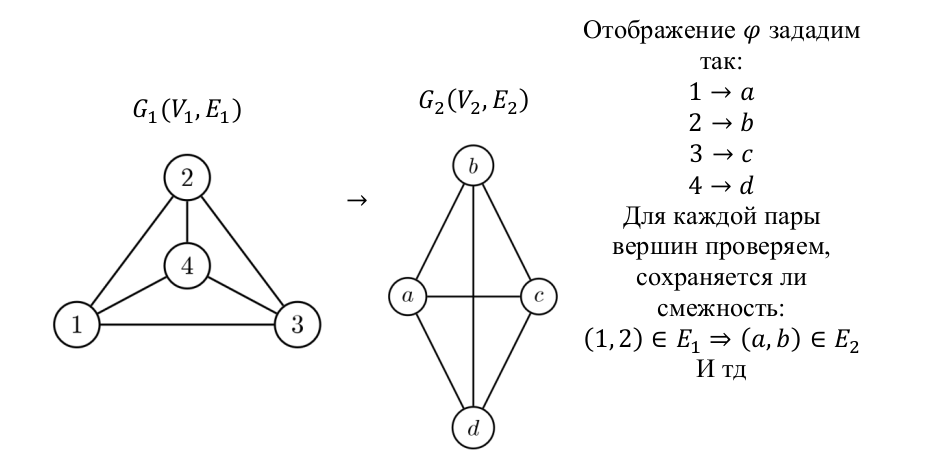
\includegraphics[scale=0.25]{3_iso.png}
\end{figure}

\begin{definition}
    \textit{Инвариантом изоморфизма графов} называется некоторое
    (обычно числовое) значение или упорядоченный набор значений,
    характеризующий структуру графа и не зависящий от способа его задания.
\end{definition}

Инвариантами графа являются:
\begin{enumerate}[left=0.0em, labelsep=1em, topsep=0.0em, itemsep=0pt, parsep=0.5em]
    \item Количество вершин
    \item Количество ребер
    \item Набор степеней вершин (упорядоченный)
    \item Определитель матрицы смежности
    \item Количество компонент связности
    \item Хроматическое число и т.д.
\end{enumerate}

Пусть $G(V,E)$ -- простой неориентированный граф.

\begin{definition}
    Дополнением графа $G$ называется граф $\overline{G}(\overline{V},\overline{E})$,
    у которого $\overline{V}=V$, в множестве $\overline{E}$ содержатся ребра полного графа,
    которых нет в множестве $E$.
\end{definition}

\begin{theorem}
    Простые графы $G$ и $H$ изоморфны тогда и только тогда, когда изоморфны их дополнения.
    \begin{align*}
        G \cong H \Leftrightarrow \overline{G} \cong \overline{H}
    \end{align*}
\end{theorem}

\begin{definition}
    Граф является самодополнительным, если он изоморфен своему дополнению.
\end{definition}

Понятие изоморфизма можно дать и для произвольных графов.

\begin{definition}
    Граф $G_1(V_1,E_1)$ и $G_2(V_2,E_2)$ \textit{изоморфны}, если $\exists$
    биективные отображения $\varphi : V_1 \rightarrow V_2$ и $h: E_1 \rightarrow E_2$
    такие, что:
    $$e = (u,v) \in E_1 \Leftrightarrow h(e) = (\varphi(u),\varphi(v)) \in E_2$$
\end{definition}

\newpage
\textbf{Гомеоморфизм графов}

\begin{definition}
    \textit{Операция подразбиения ребра} $(u, v)$ состоит в удалении этого
    ребра, добавлении вершины $\omega$ и рёбер $(u, \omega)$ и $(\omega, v)$.
\end{definition}

\begin{definition}
    Граф $G_2$ называется \textit{подразбиением} графа $G_1$, если его можно
    получить из графа $G_1$ путём последовательного применения операции
    подразбиения рёбер (сам граф тоже является своим подразбиением).
\end{definition}

\begin{figure}[h]
    \centering
    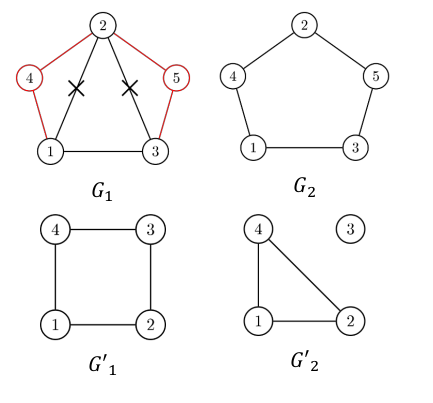
\includegraphics[scale=0.4]{3_2.png}
\end{figure}

Графы $G_1$ и $G_2$ на рисунке гомеоморфны, потому что их подразбиения
изоморфны.

Покажем, что графы ${G_1}'$ и ${G_2}'$ не гомеоморфны.

При любой операции подразбиения ребер появляются вершины степени 2, у
остальных вершин степень не меняется. В графе ${G_2}'$ есть вершина степени 0,
она останется такой при любом количестве операций подразбиения ребер. В
графе ${G_1}'$ все вершины имеют степень 2. При любом количестве операций
подразбиения ребер появятся вершины степени 2, у имеющихся вершин
степень не изменится. Это значит, что любые подразбиения графов не
являются изоморфными, поэтому графы ${G_1}'$ и ${G_2}'$ на рисунке не
гомеоморфны.
	\section{Маршруты, цепи, циклы в графе. Метрические характеристики графа. Найти эксцентриситет 
вершины указанного графа, радиус, диаметр графа, центральные и периферийные вершины 
указанного графа.}
	\section{Алгоритмы обхода графа в глубину и ширину.}

\begin{definition}
    Обход графа (поиск на графе) –- это процесс систематического просмотра
    всех ребер или вершин графа с целью отыскания ребер или вершин,
    удовлетворяющих некоторому условию.
\end{definition}

\begin{definition}
    Поиск в ширину (BFS) нужен для нахождения расстояний между вершин в связном графе.
    Алгоритм по принципу напоминает "пожар".
\end{definition}

Алгоритм поиска в ширину:
\begin{enumerate}[left=0.0em, labelsep=1em, topsep=0em, itemsep=0pt, parsep=0.5em]
    \item Все вершины окрашиваются в белый цвет.
    \item Выбирается первая вершина, раскрашивается в черный цвет и заносится в очередь.
    \item Посещается первая вершина из очереди. Все смежные с ней белые вершины
    раскрашиваются в черный цвет и заносятся в очередь. После этого эта вершина удаляется
    из очереди.
    \item Повторяется шаг 3 до тех пор пока очередь не пуста.
\end{enumerate}

\begin{figure}[h]
    \centering
    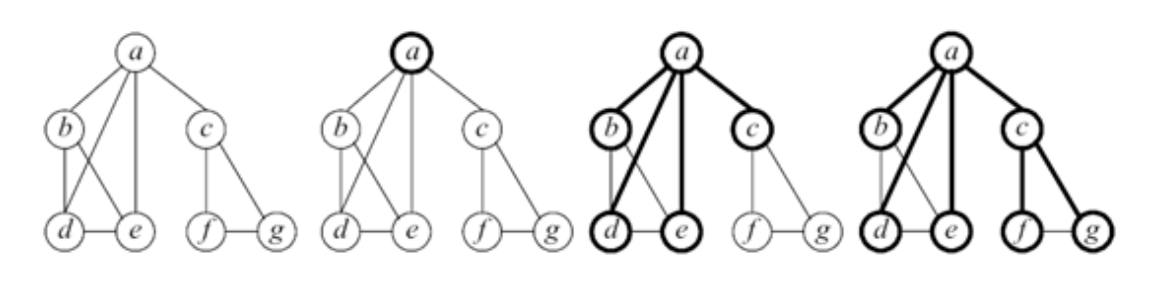
\includegraphics[width=\textwidth]{5_bfs.png}
\end{figure}

Сложность поиска в ширину при нематричном представлении графа
равна $O(n+m)$, так как рассматриваются все n вершин и m ребер.
Использование матрицы смежности приводит к оценке $O(n^2)$.

Если граф не является связным, то нужно добавить шаг 5, в
котором написать, что нужно повторять 2 шаг до тех пор, пока в графе не
останется белых вершин.

Если сначала присвоить первой вершине значение 0, потом
смежным с ней вершинам 0+1 =1, и так далее, то в итоге для каждой
вершины будет найдено расстояние от первой вершины.
\newpage

\begin{definition}
    Поиск в глубину (DFS) исследует конкретную ветку в графе и только потом переходит к другой (если они остануться нерассмотренными).
\end{definition}

Вершины графа могут быть раскрашены в три цвета: белый цвет означает, что
в вершине еще не были, серый – что в вершине были, но еще вернемся, черный
– что были и больше не рассматриваем.

Алгоритм поиска в глубину:
\begin{enumerate}[left=0.0em, labelsep=1em, topsep=0em, itemsep=0pt, parsep=0.5em]
    \item Всем вершинам графа присваиваем белый цвет.
    \item Выбираем первую вершину и раскрашиваем в серый цвет.
    \item Для последней раскрашенной в серый цвет вершины выбираем белую
    смежную ей вершину (если такая вершина есть), раскрашиваем ее в серый цвет
    и переходим к шагу 3.
    \item Повторяем шаг 3 до тех пор, пока все вершины не будут раскрашены в
    черный цвет.
\end{enumerate}

Если для рассматриваемой вершины белых смежных с ней вершин нет, то
рассматриваемую вершину раскрашиваем в черный цвет и переходим к шагу
3.

\begin{figure}[h]
    \centering
    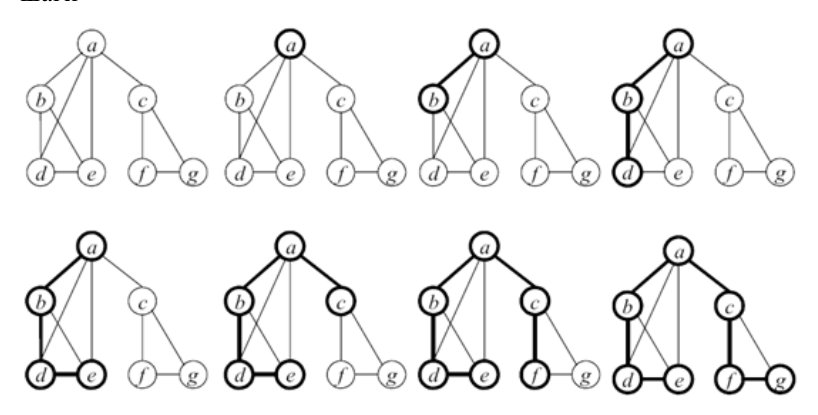
\includegraphics[width=\textwidth]{5_dfs.png}
\end{figure}

Временная сложность алгоритма зависит от представления графа. Если
применена матрица смежности, то временная сложность равна $O(n^2)$, а если
нематричное представление -- $O(n+m)$: рассматриваются все вершины и все ребра.

\end{document}